% \definecolor{temoin}{HTML}{D9EAD3}
% \definecolor{parent}{HTML}{FFF2CC}
% \definecolor{epoux}{HTML}{FCE5CD}
% \definecolor{epouse}{HTML}{D9D2E9}
\definecolor{lightgrey}{gray}{0.9}


\colorlet{temoin}{teal!80!white!50}
\colorlet{parent}{yellow!80!white!50}
\colorlet{epoux}{orange!80!white!50}
\colorlet{epouse}{purple!80!white!50}


\newcommand{\simple}[1][0]{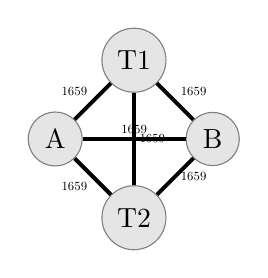
\begin{tikzpicture}[node distance=3cm, auto]
        \node[shape=circle,draw=gray, fill=lightgrey] (A) at (0,1) {A};
        \node[shape=circle,draw=gray, fill=lightgrey] (B) at (2,1) {B};
        \node[shape=circle,draw=gray, fill=lightgrey] (T1) at (1,2) {T1};
        \node[shape=circle,draw=gray, fill=lightgrey] (T2) at (1,0) {T2};
    
        \begin{scope}[every node/.style={scale=.5}]
            \path [line width=0.5mm]
            (A)  edge node [color=black] {\small 1659} (B)
            (T1) edge node [color=black] {\small 1659} (T2)
            (T1) edge node [above left, color=black] {\small 1659} (A)
            (T1) edge node [color=black] {\small 1659} (B)
            (T2) edge node [color=black] {\small 1659} (A)
            (T2) edge node [right, color=black] {\small 1659} (B); 
        \end{scope}
    \end{tikzpicture}}
    

\newcommand{\noParents}[1][0]{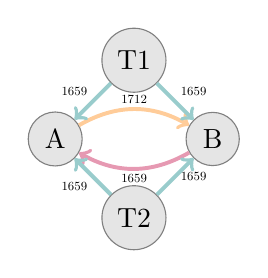
\begin{tikzpicture}[->, node distance=3cm, auto]
        \node[shape=circle,draw=gray, fill=lightgrey] (A) at (0,1) {A};
        \node[shape=circle,draw=gray, fill=lightgrey] (B) at (2,1) {B};
        \node[shape=circle,draw=gray, fill=lightgrey] (T1) at (1,2) {T1};
        \node[shape=circle,draw=gray, fill=lightgrey] (T2) at (1,0) {T2};
    
        \begin{scope}[every node/.style={scale=.5}]
            \path [line width=0.5mm] (A) edge [bend left, color=epoux] node [color=black] {\small 1712} (B)
            (B) edge [bend left, color=epouse] node [color=black] {\small 1659} (A)
            (T1) edge [color=temoin] node [above left, color=black] {\small 1659} (A)
            (T1) edge [color=temoin] node [color=black] {\small 1659} (B)
            (T2) edge [color=temoin] node [color=black] {\small 1659} (A)
            (T2) edge [color=temoin] node [right, color=black] {\small 1659} (B); 
        \end{scope}
    \end{tikzpicture}}
    
% \newcommand{\bipartiteNoParents}[1]{\begin{tikzpicture}[, node distance=3cm, auto, scale=#1]
\newcommand{\bipartiteNoParents}[1][0]{\begin{tikzpicture}[, node distance=3cm, auto]
        \node[shape=circle,draw=gray, fill=lightgrey] (A) at (0,3) {H};
        \node[shape=circle,draw=gray, fill=lightgrey] (B) at (0,1) {W};
        
        \node[shape=circle,draw=gray, fill=lightgrey] (T1) at (3,3) {T1};
        \node[shape=circle,draw=gray, fill=lightgrey] (T2) at (3,1) {T2};
        
        \node[shape=rectangle,draw=gray, align=center,fill=lightgrey] (D) at (1.5,2) {M \\[0.5em] \small 1659};
        \draw (D.west) -- (D.east);
    
        \begin{scope}[every node/.style={scale=.5}]
            \path [line width=0.5mm] (A) edge [color=epoux] (D)
            (B) edge [color=epouse] (D)
            (T1) edge [color=temoin] (D)
            (T2) edge [color=temoin] (D);
        \end{scope}
        \end{tikzpicture}}

\newcommand{\unipartiteParents}[1][0]{
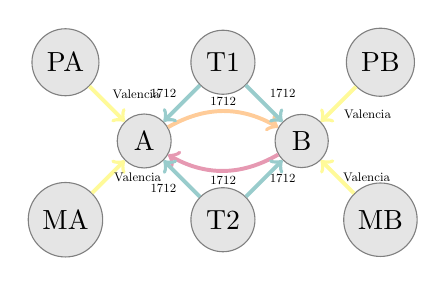
\begin{tikzpicture}[->, node distance=3cm, auto]
        \node[shape=circle,draw=gray, fill=lightgrey] (A) at (2,1) {A};
        \node[shape=circle,draw=gray, fill=lightgrey] (B) at (4,1) {B};
        
        \node[shape=circle,draw=gray, fill=lightgrey] (T1) at (3,2) {T1};
        \node[shape=circle,draw=gray, fill=lightgrey] (T2) at (3,0) {T2};
        
        \node[shape=circle,draw=gray, fill=lightgrey] (PA) at (1,2) {PA};
        \node[shape=circle,draw=gray, fill=lightgrey] (MA) at (1,0) {MA};
        
        \node[shape=circle,draw=gray, fill=lightgrey] (PB) at (5,2) {PB};
        \node[shape=circle,draw=gray, fill=lightgrey] (MB) at (5,0) {MB};
    
    \begin{scope}[every node/.style={scale=.5}]
        \path [line width=0.5mm] (A) edge [bend left, color=epoux] node [color=black] {\small 1712} (B)
        (B) edge [bend left, color=epouse] node [color=black] {\small 1712} (A)
        (T1) edge [color=temoin] node [above left, color=black] {\small 1712} (A)
        (T1) edge [color=temoin] node [color=black] {\small 1712} (B)
        (T2) edge [color=temoin] node [color=black] {\small 1712} (A)
        (T2) edge [color=temoin] node [right, color=black] {\small 1712} (B)
        (PA) edge [color=parent] node [color=black] {\small Valencia} (A)
        (MA) edge [color=parent] node [right, color=black] {\small Valencia} (A)
        (PB) edge [color=parent] node [color=black] {\small Valencia} (B)
        (MB) edge [color=parent] node [right, color=black] {\small Valencia} (B);
    \end{scope}
    \end{tikzpicture}
}

\newcommand{\bipartiteParents}[1]{
\begin{tikzpicture}[, node distance=3cm, auto, scale=#1]
        \node[shape=circle,draw=gray, fill=lightgrey] (A) at (0,3) {H};
        \node[shape=circle,draw=gray, fill=lightgrey] (T1) at (0,2) {T1};
        
        \node[shape=circle,draw=gray, fill=lightgrey] (T2) at (0,1) {T2};
        \node[shape=circle,draw=gray, fill=lightgrey] (B) at (0,0) {W};
        
        \node[shape=rectangle,draw=gray, align=center, fill=lightgrey] (D) at (1.5,1.5) {M \\[0.5em] \tiny 1761};
        
        \node[shape=rectangle,draw=gray, align=center, fill=lightgrey] (BA) at (1.5,3) {BA \\[0.5em] \tiny Valencia};
        \node[shape=rectangle,draw=gray, align=center, fill=lightgrey] (BB) at (1.5,0) {BB \\[0.5em] \tiny Valencia};
        
        \draw (D.west) -- (D.east);
        \draw (BA.west) -- (BA.east);
        \draw (BB.west) -- (BB.east);
        
        \node[shape=circle,draw=gray, fill=lightgrey] (PA) at (3,3) {HF};
        \node[shape=circle,draw=gray, fill=lightgrey] (MA) at (3,2) {HM};
        \node[shape=circle,draw=gray, fill=lightgrey] (PB) at (3,1) {WF};
        \node[shape=circle,draw=gray, fill=lightgrey] (MB) at (3,0) {WM};
    
    \begin{scope}[every node/.style={scale=.5}]
        \path [line width=0.5mm] (A) edge [color=epoux] (D)
        (B) edge [color=epouse] (D)
        (T1) edge [color=temoin] (D)
        (T2) edge [color=temoin] (D)
        (PA) edge [color=parent] (BA)
        (MA) edge [color=parent] (BA)
        (PB) edge [color=parent] (BB)
        (MB) edge [color=parent] (BB)
        (A) edge [color=parent] (BA)
        (B) edge [color=parent] (BB);
    \end{scope}
    \end{tikzpicture}
}



\iffalse
\begin{figure}
    \centering
    
%     \begin{subfigure}{0.5\columnwidth}
%     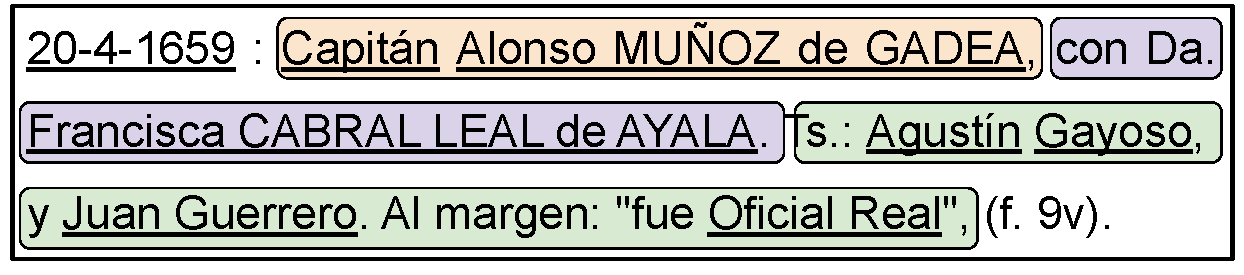
\includegraphics[width=\columnwidth]{Figures/marriageDocumentnoParents.pdf} 
%     % \caption{First, an exciting contribution by unknown artist.}
%   \end{subfigure}
%   \begin{subfigure}{0.32\columnwidth}
%     \bipartiteNoParents{1}
% %   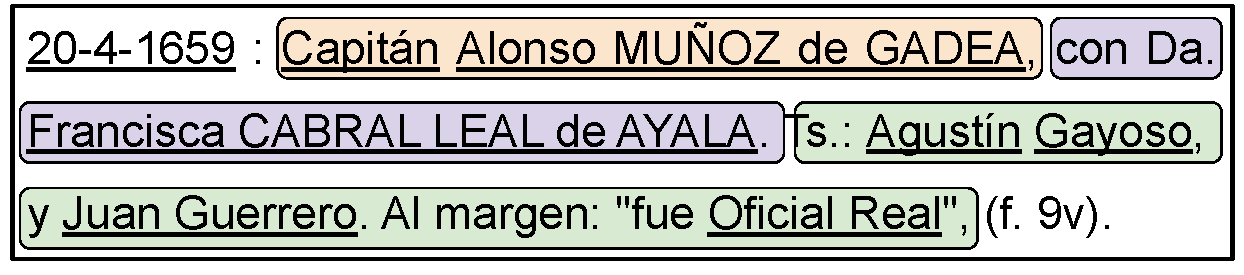
\includegraphics[width=\linewidth]{Figures/marriageDocumentnoParents.pdf} 
% %   \resizebox{0.5\textwidth}{!}{
% %     \bipartiteNoParents{1}
% % }%
%     % \caption{Second, an anonymous mystery.}
%   \end{subfigure}
%   \begin{subfigure}{0.5\columnwidth}
%     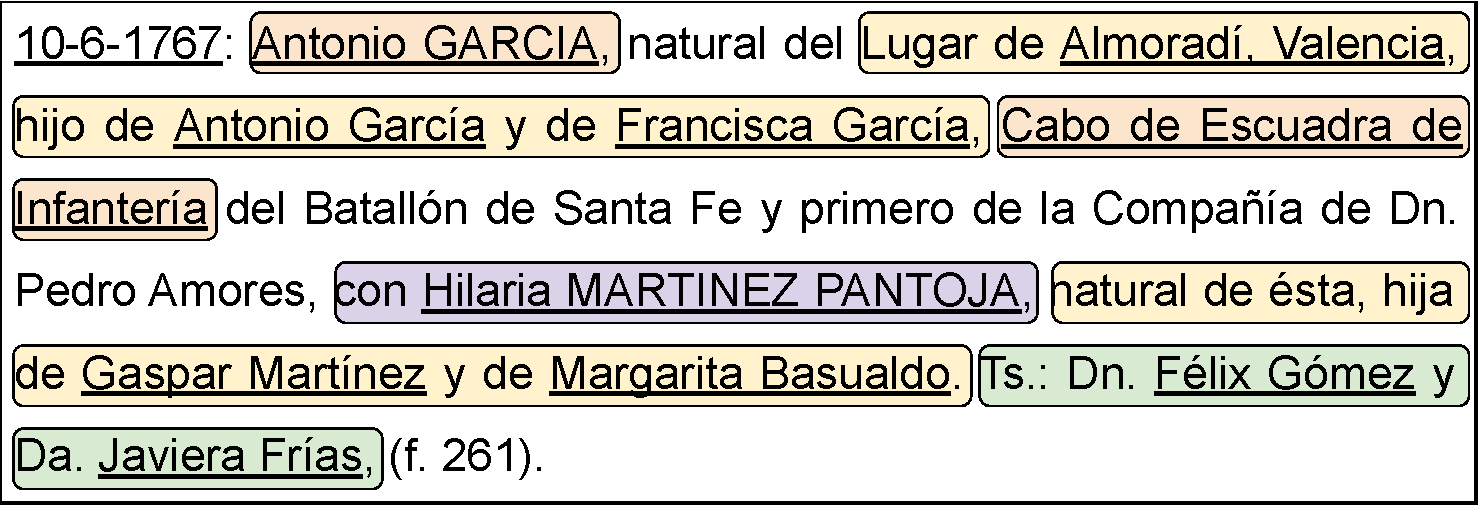
\includegraphics[width=\linewidth]{Figures/marriageDocument.pdf} 
%   \end{subfigure}
%   \begin{subfigure}{0.3\columnwidth}
%     \bipartiteParents{1}
%   \end{subfigure}
  
  
  \begin{subfigure}{.23\textwidth}
    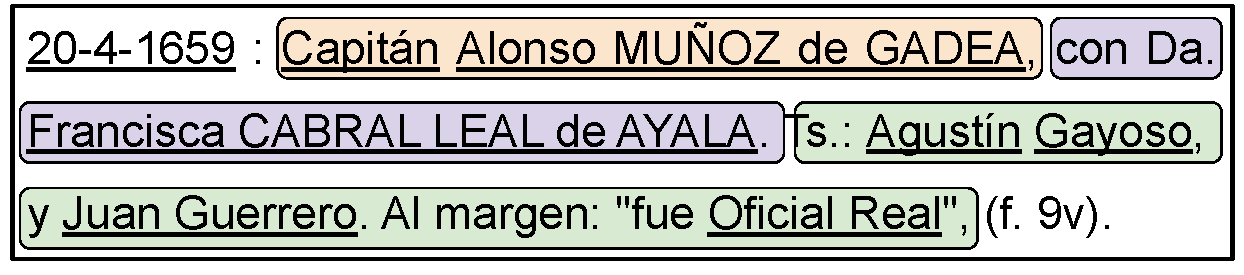
\includegraphics[width=\linewidth]{Figures/marriageDocumentnoParents.pdf}
    \caption{}
  \end{subfigure}
  \begin{subfigure}{.23\textwidth}
    \centering
    \bipartiteNoParents{1}
  \end{subfigure}
  \begin{subfigure}{.23\textwidth}
    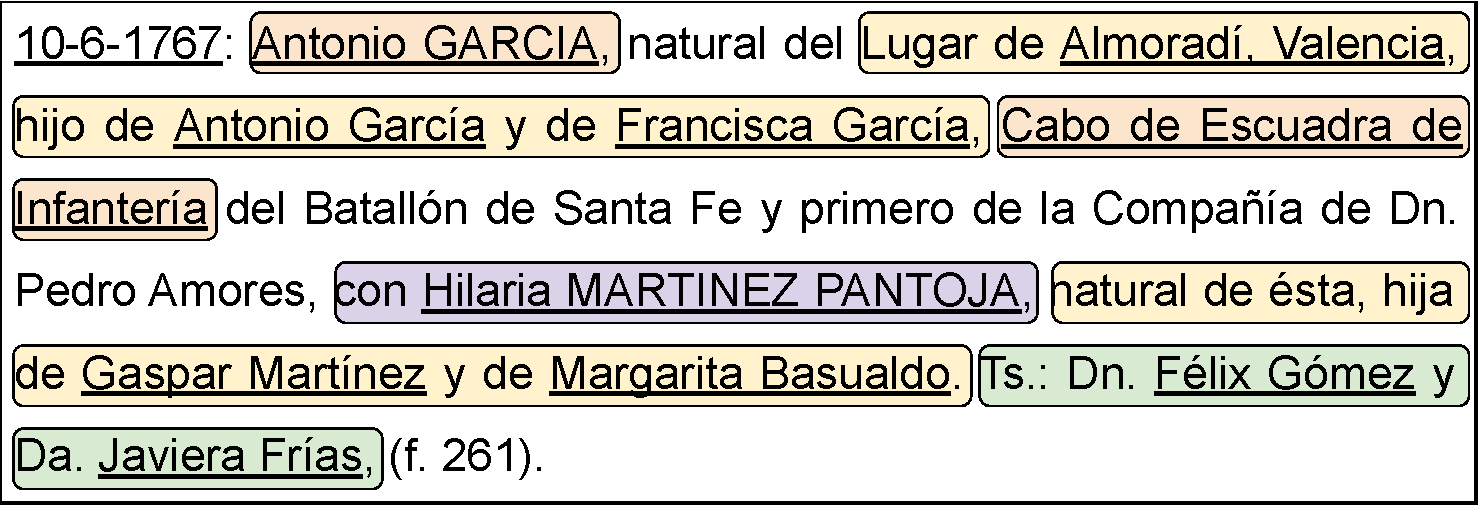
\includegraphics[width=\linewidth]{Figures/marriageDocument.pdf} 
    \caption{}
    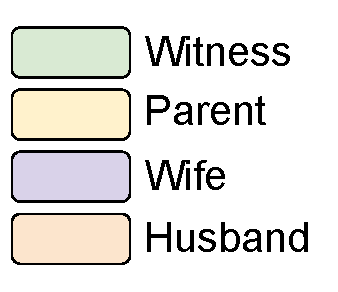
\includegraphics[scale=0.2,left]{Figures/MarriageLegend.pdf}
  \end{subfigure}
  \centering
  \begin{subfigure}{.23\textwidth}
    \bipartiteParents{1}
  \end{subfigure}
    
    
    % 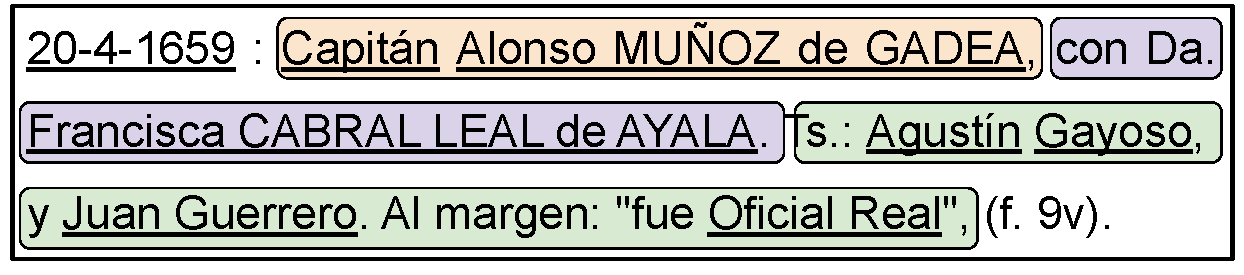
\includegraphics[width=0.49\linewidth]{Figures/marriageDocumentnoParents.pdf} 
    % \bipartiteNoParents{1}
    % % \subfigure[]{\bipartiteNoParents{0.6}} 

    % 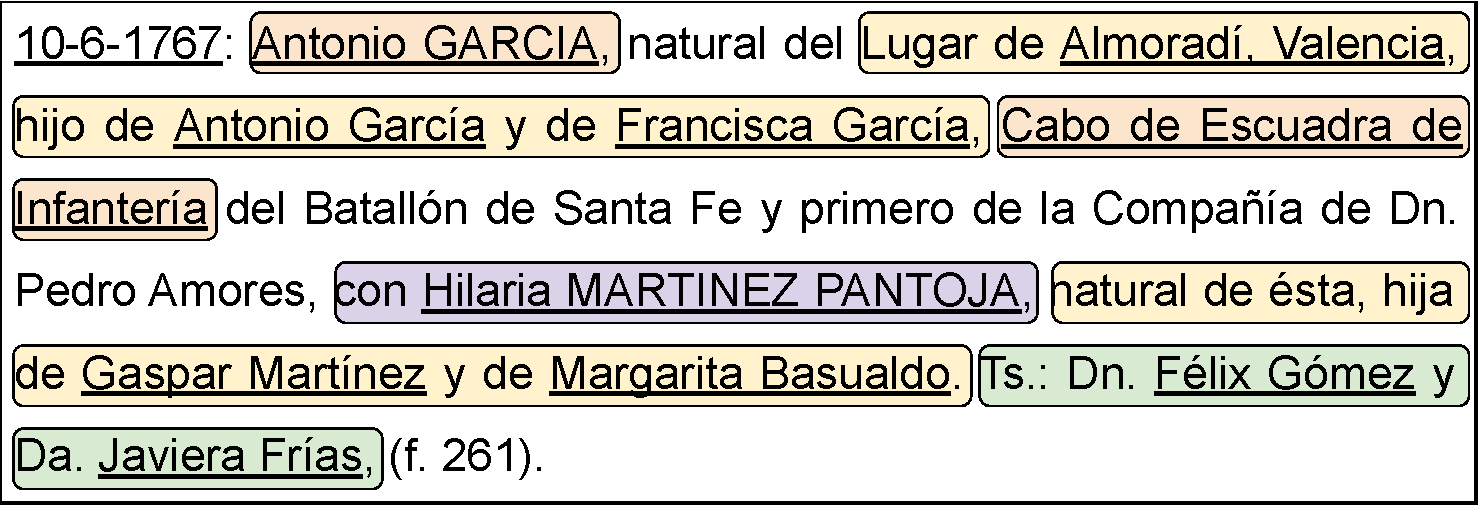
\includegraphics[width=0.49\linewidth]{Figures/marriageDocument.pdf}
    % \bipartiteParents{1}
    
    \caption{Transformation of annotated marriage acts from use case \zacarias\ into our proposed model. The acts can refers to parent relationships (b) or not (a). Each color represent a relationship between a person and an event. Additional information on the persons or the events are underlined and stored in the nodes as attributes. The network is a concrete representation of the events mentioned in the original sources. H: Husband, W: wife, T1,T2: witnesses, M: marriage act, HF, HM, WF, WM: husband/wife's father/mother.
    % \jdf{Tu peux expliquer les A, B, T1, T2, PA, MA, PB, MB?}
    }\label{tab:MarriageModel}
\end{figure}
\fi


% \definecolor{associate}{rgb}{1, 0, 1}
% \definecolor{guarantor}{rgb}{0, 0, 1.0}
% \definecolor{approbator}{rgb}{0, 1, 0}

\colorlet{associate}{orange!80!white!50}
\colorlet{guarantor}{blue!80!white!50}
\colorlet{approbator}{olive!80!white!50}

% \colorlet{approbator}{LimeGreen}

\newcommand{\simplePiemont}[1][0]{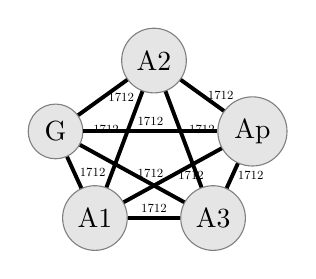
\begin{tikzpicture}[node distance=3cm, auto]
        \node[shape=circle,draw=gray, fill=lightgrey] (A1) at (2,1) {A1};
        \node[shape=circle,draw=gray, fill=lightgrey] (A2) at (2.75,3) {A2};
        \node[shape=circle,draw=gray, fill=lightgrey] (A3) at (3.5,1) {A3};
        \node[shape=circle,draw=gray, fill=lightgrey] (G) at (1.5,2.1) {G};
        \node[shape=circle,draw=gray, fill=lightgrey] (Ap) at (4,2.1) {Ap};
    
        \begin{scope}[every node/.style={scale=.5}]
            \path [line width=0.5mm]
            (A1) edge node [above left, color=black] {\small 1712} (A2)
            (A1) edge node [color=black] {\small 1712} (A3)
            (A2) edge node [color=black] {\small 1712} (A3)
            (G) edge node [right, color=black] {\small 1712} (A1)
            (G) edge node [right, color=black] {\small 1712} (A2) 
            (G) edge node [right, color=black] {\small 1712} (A3)
            (Ap) edge node [right, color=black] {\small 1712} (A1)
            (Ap) edge node [right, color=black] {\small 1712} (A2) 
            (Ap) edge node [right, color=black] {\small 1712} (A3)
            (G) edge node [color=black] {\small 1712} (Ap); 
        \end{scope}
    \end{tikzpicture}}

\newcommand{\unipartitePiemont}[1][0]{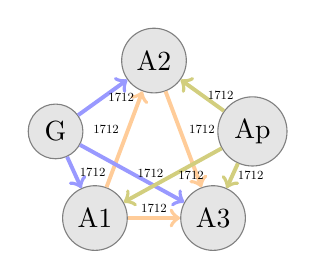
\begin{tikzpicture}[->, node distance=3cm, auto]
        \node[shape=circle,draw=gray, fill=lightgrey] (A1) at (2,1) {A1};
        \node[shape=circle,draw=gray, fill=lightgrey] (A2) at (2.75,3) {A2};
        \node[shape=circle,draw=gray, fill=lightgrey] (A3) at (3.5,1) {A3};
        \node[shape=circle,draw=gray, fill=lightgrey] (G) at (1.5,2.1) {G};
        \node[shape=circle,draw=gray, fill=lightgrey] (Ap) at (4,2.1) {Ap};
    
        \begin{scope}[every node/.style={scale=.5}]
            \path [line width=0.5mm]
            (A1) edge [color=associate] node [above left, color=black] {\small 1712} (A2)
            (A1) edge [color=associate] node [color=black] {\small 1712} (A3)
            (A2) edge [color=associate] node [color=black] {\small 1712} (A3)
            (G) edge [color=guarantor] node [right, color=black] {\small 1712} (A1)
            (G) edge [color=guarantor] node [right, color=black] {\small 1712} (A2) 
            (G) edge [color=guarantor] node [right, color=black] {\small 1712} (A3)
            (Ap) edge [color=approbator] node [right, color=black] {\small 1712} (A1)
            (Ap) edge [color=approbator] node [right, color=black] {\small 1712} (A2) 
            (Ap) edge [color=approbator] node [right, color=black] {\small 1712} (A3); 
        \end{scope}
    \end{tikzpicture}}
    
    
\newcommand{\bipartitePiemont}[1][0]{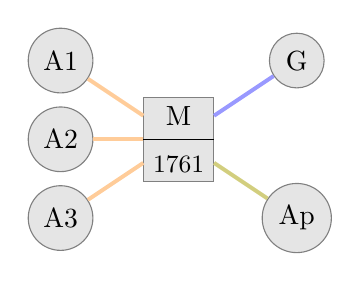
\begin{tikzpicture}[, node distance=3cm, auto]
        \node[shape=circle,draw=gray, fill=lightgrey] (A1) at (0,3) {A1};
        \node[shape=circle,draw=gray, fill=lightgrey] (A2) at (0,2) {A2};
        \node[shape=circle,draw=gray, fill=lightgrey] (A3) at (0,1) {A3};
        
        \node[shape=circle,draw=gray, fill=lightgrey] (G) at (3,3) {G};
        \node[shape=circle,draw=gray, fill=lightgrey] (Ap) at (3,1) {Ap};
        
        \node[shape=rectangle,draw=gray, align=center,fill=lightgrey] (D) at (1.5,2) {M \\[0.5em] \small 1761};
        \draw (D.west) -- (D.east);
    
        \begin{scope}[every node/.style={scale=.5}]
            \path [line width=0.5mm] (A1) edge [color=associate] (D)
            (A2) edge [color=associate] (D)
            (A3) edge [color=associate] (D)
            (G) edge [color=guarantor] (D)
            (Ap) edge [color=approbator] (D);
        \end{scope}
        \end{tikzpicture}}
        
        

% \definecolor{father}{rgb}{1, 0, 1}
\colorlet{father}{red!80!white!50}
\colorlet{mother}{green!80!white!50}
\colorlet{child}{blue!80!white!50}

% \definecolor{mother}{rgb}{0, 0, 1.0}
% \definecolor{child}{rgb}{0, 1, 0}


\newcommand{\birthSimple}[1][0]{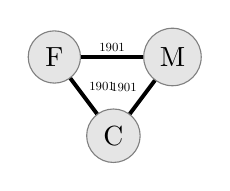
\begin{tikzpicture}[, node distance=3cm, auto]
        \node[shape=circle,draw=gray, fill=lightgrey] (F) at (0,1) {F};
        \node[shape=circle,draw=gray, fill=lightgrey] (M) at (1.5,1) {M};
        \node[shape=circle,draw=gray, fill=lightgrey] (C) at (0.75,0) {C};
    
        \begin{scope}[every node/.style={scale=.5}]
            \path [line width=0.5mm] (F) edge [color=black] node [above right, color=black] {\small 1901} (C)
            (M) edge node [above left, color=black] {\small 1901} (C)
            (F) edge node [color=black] {\small 1901} (M);
        \end{scope}
        \end{tikzpicture}}

\newcommand{\birthUnipartite}[1][0]{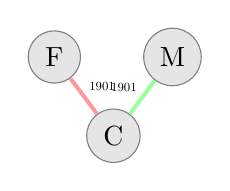
\begin{tikzpicture}[, node distance=3cm, auto]
        \node[shape=circle,draw=gray, fill=lightgrey] (F) at (0,1) {F};
        \node[shape=circle,draw=gray, fill=lightgrey] (M) at (1.5,1) {M};
        \node[shape=circle,draw=gray, fill=lightgrey] (C) at (0.75,0) {C};
    
        \begin{scope}[every node/.style={scale=.5}]
            \path [line width=0.5mm] (F) edge [color=father] node [above right, color=black] {\small 1901} (C)
            (M) edge [color=mother] node [above left, color=black] {\small 1901} (C);
        \end{scope}
        \end{tikzpicture}}
        
\newcommand{\birthBipartite}[1][0]{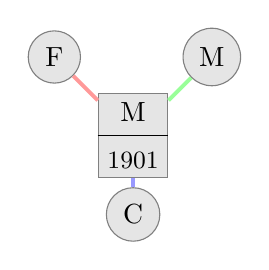
\begin{tikzpicture}[, node distance=3cm, auto]
        \node[shape=circle,draw=gray, fill=lightgrey] (F) at (0,2) {F};
        \node[shape=circle,draw=gray, fill=lightgrey] (M) at (2,2) {M};
        \node[shape=rectangle,draw=gray, align=center,fill=lightgrey] (D) at (1,1) {M \\[0.5em] \small 1901};
        \draw (D.west) -- (D.east);
        \node[shape=circle,draw=gray, fill=lightgrey] (C) at (1,0) {C};
    
        \begin{scope}[every node/.style={scale=.5}]
            \path [line width=0.5mm] (F) edge [color=father] (D)
            (M) edge [color=mother] (D)
            (D) edge [color=child] (C);
        \end{scope}
        \end{tikzpicture}}
        
        
    %      \hline Original Document & Co-occurrence & Unipartite representation & Proposed model \\
    % \hline \centering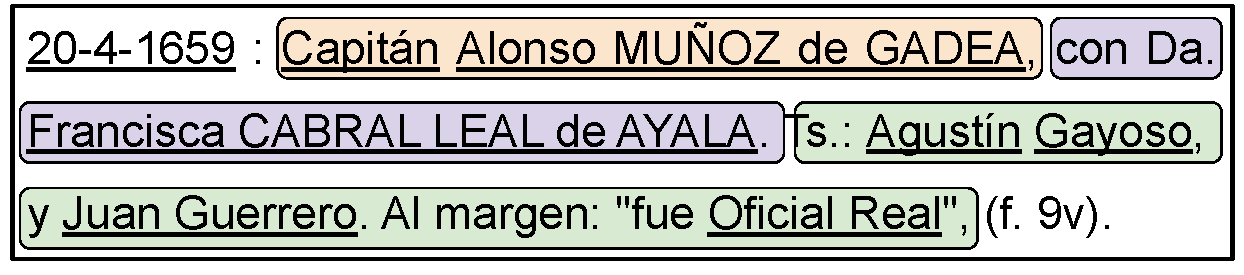
\includegraphics[scale=0.3]{Figures/marriageDocumentnoParents} & \simple & \centering\noParents & \bipartiteNoParents \\
    % \hline doc & \simplePiemont & \centering\unipartitePiemont & \bipartitePiemont \\
    % \hline doc & \birthSimple